\documentclass[12pt,a4paper]{article}

% ─── 1. PACKAGES ──────────────────────────────────────────────────────────────
\usepackage[utf8]{inputenc}
\usepackage[T1]{fontenc}
\usepackage{amsmath, amssymb}
\usepackage{geometry}
\usepackage{graphicx}
\usepackage{xcolor}
\usepackage{listings}
\usepackage{hyperref}
\usepackage{booktabs}
\usepackage{enumitem}
\usepackage{tcolorbox}
\usepackage{mdframed}
\usepackage{fancyhdr}
\usepackage{titlesec}
\usepackage{tikz} % Ditambahkan untuk menggambar figure Automata
\usetikzlibrary{automata, positioning, arrows.meta}

% Font Settings
\usepackage{newtxtext,newtxmath} % Times New Roman
\usepackage{courier}             % Courier New untuk kode

\geometry{margin=2.5cm}

% ─── 2. WARNA TEMA ────────────────────────────────────────────────────────────
\definecolor{codebg}{RGB}{245,247,250}
\definecolor{codeframe}{RGB}{180,195,215}
\definecolor{keywordcolor}{RGB}{0,112,192}
\definecolor{commentcolor}{RGB}{100,160,100}
\definecolor{stringcolor}{RGB}{180,70,50}
\definecolor{notebg}{RGB}{255,249,230}
\definecolor{noteframe}{RGB}{230,180,50}
\definecolor{tipbg}{RGB}{230,245,235}
\definecolor{tipframe}{RGB}{50,160,90}
\definecolor{sectioncolor}{RGB}{30,80,150}

% ─── 3. STYLE SECTION & TOC ───────────────────────────────────────────────────
\titleformat{\section}{\Large\bfseries\color{sectioncolor}}{}{0em}{\thesection\quad}[\titlerule]
\titleformat{\subsection}{\large\bfseries\color{sectioncolor!80}}{}{0em}{\thesubsection\quad}

% Style Table of Contents
\usepackage{tocloft}
\renewcommand{\cftsecleader}{\cftdotfill{\cftdotsep}}
\renewcommand{\cftsecfont}{\bfseries\color{sectioncolor}}

% ─── 4. LISTINGS (CODE STYLE) ─────────────────────────────────────────────────
\lstdefinestyle{customstyle}{
  basicstyle=\ttfamily\small,
  backgroundcolor=\color{codebg},
  frame=single,
  rulecolor=\color{codeframe},
  keywordstyle=\bfseries\color{keywordcolor},
  commentstyle=\itshape\color{commentcolor},
  stringstyle=\color{stringcolor},
  numbers=left,
  numberstyle=\tiny\color{gray},
  breaklines=true,
  tabsize=4,
  showstringspaces=false
}
\lstset{style=customstyle}

% ─── 5. KOTAK CATATAN (MD-FRAME) ──────────────────────────────────────────────
\newmdenv[
  backgroundcolor=notebg, linecolor=noteframe, linewidth=2pt,
  leftline=true, topline=false, rightline=false, bottomline=false,
  innerleftmargin=10pt, innertopmargin=6pt, innerbottommargin=6pt, skipabove=8pt
]{notebox}

\newmdenv[
  backgroundcolor=tipbg, linecolor=tipframe, linewidth=2pt,
  leftline=true, topline=false, rightline=false, bottomline=false,
  innerleftmargin=10pt, innertopmargin=6pt, innerbottommargin=6pt, skipabove=8pt
]{tipbox}

% ─── 6. HEADER & FOOTER ───────────────────────────────────────────────────────
\pagestyle{fancy}
\fancyhf{}
\fancyhead[L]{\small\textit{Teori Bahasa dan Automata}}
\fancyhead[R]{\small\textit{noteify -- Modul Deterministic Finite Automata}}
\fancyfoot[C]{\thepage}
\renewcommand{\headrulewidth}{0.4pt}

% ─── 7. DATA COVER ────────────────────────────────────────────────────────────
\title{
  {\LARGE\bfseries TEORI BAHASA DAN AUTOMATA}\\[0.5em]
  {\large Modul Pembelajaran: Deterministic Finite Automata (DFA)}\\[0.8em]
  {\normalsize Modul komprehensif mengenai konsep dasar, definisi formal, struktur loop, dan contoh perancangan DFA.}
}
\author{}
\date{}

% ==============================================================================
\begin{document}

\maketitle
\thispagestyle{fancy}
\tableofcontents
\newpage

% ─── KONTEN MATERI ─────────────────────────────────────────────────────────────

\section{Konsep Dasar Deterministic Finite Automata (DFA)}

\subsection{Pengantar dan Prinsip Kerja DFA}
\textit{Deterministic Finite Automaton} (DFA) adalah mesin abstrak yang digunakan untuk mengenali pola atau bahasa reguler[cite: 1, 3]. Mesin ini beroperasi dengan membaca sekumpulan karakter (\textit{String}) dari sebuah pita masukan (\textit{Input Tape}) satu per satu dari kiri ke kanan[cite: 1]. Hasil akhir dari pemrosesan ini hanya memiliki dua kemungkinan: mesin menerima (\textit{Accept}) string tersebut, atau menolaknya (\textit{Reject})[cite: 1].

Sifat fundamental dari DFA adalah \textbf{Determinisme}[cite: 1]. Artinya, jika mesin berada di suatu \textit{state} dan menerima sebuah simbol input tertentu, maka arah perpindahan \textit{state} selanjutnya sudah dapat dipastikan secara mutlak[cite: 1]. Tidak ada keraguan atau percabangan ganda untuk satu simbol input yang sama[cite: 1]. Misalnya, jika mesin berada di state A dan membaca angka "1", ia hanya memiliki satu jalan, yaitu menuju state B[cite: 1].

\begin{notebox}
\textbf{Karakteristik Determinisme pada DFA}
\begin{itemize}
    \item \textbf{Kepastian Arah:} Hanya mempunyai tepat satu \textit{state} tujuan untuk setiap kombinasi \textit{state} asal dan input[cite: 1].
    \item \textbf{Kewajiban Transisi:} Setiap \textit{state} di dalam DFA \textbf{wajib} memiliki transisi keluar untuk setiap simbol yang ada di dalam alfabet (himpunan input)[cite: 1].
\end{itemize}
\end{notebox}

\subsection{Struktur Diagram Transisi DFA}
Secara visual, DFA digambarkan menggunakan graf berarah yang disebut diagram transisi. Terdapat lima elemen visual utama dalam diagram ini:
\begin{enumerate}
    \item \textbf{Initial State}: Merupakan state awal tempat mesin mulai membaca string, ditandai dengan anak panah yang masuk tanpa state asal[cite: 1].
    \item \textbf{State}: Merepresentasikan kedudukan atau memori mesin pada suatu waktu, digambarkan dengan lingkaran[cite: 1].
    \item \textbf{Transition}: Arah perpindahan antar state, digambarkan dengan garis berpanah[cite: 1].
    \item \textbf{Input}: Simbol yang dituliskan di atas garis transisi, bertindak sebagai pemicu perpindahan state[cite: 1].
    \item \textbf{Final State}: Kedudukan akhir penerimaan, digambarkan dengan lingkaran ganda (\textit{double circle})[cite: 1]. Sebuah DFA dapat memiliki lebih dari satu \textit{final state} (\textit{multi final state})[cite: 1].
\end{enumerate}

\begin{figure}[h]
    \centering
    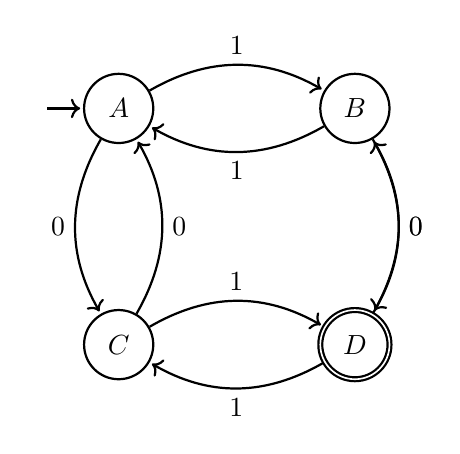
\begin{tikzpicture}[shorten >=1pt,node distance=3cm,on grid,auto, thick]
       \node[state,initial,initial text=] (A) {$A$};
       \node[state] (B) [right=of A] {$B$};
       \node[state] (C) [below=of A] {$C$};
       \node[state,accepting] (D) [right=of C] {$D$};

       \path[->] 
       (A) edge [bend left] node {1} (B)
           edge [bend right] node [swap] {0} (C)
       (B) edge [bend left] node {1} (A)
           edge [bend left] node {0} (D)
       (C) edge [bend right] node [swap] {0} (A)
           edge [bend left] node {1} (D)
       (D) edge [bend left] node {1} (C)
           edge [bend right] node [swap] {0} (B);
    \end{tikzpicture}
    \caption{Contoh Struktur Diagram Transisi DFA}
\end{figure}

\subsection{Syarat Diterima dan Ditolaknya String}
Proses membaca input disebut \textit{scanning}. Head mesin akan membaca satu per satu karakter hingga pita kosong (\textit{empty tape} atau \textit{input finished})[cite: 1].
\begin{itemize}
    \item \textbf{Diterima (Accept):} String diterima jika dan hanya jika semua input string telah selesai diperiksa dan mesin berhenti tepat pada salah satu \textit{final state}[cite: 1].
    \item \textbf{Ditolak (Reject):} String ditolak jika setelah semua input habis dibaca, mesin berhenti di state yang \textbf{bukan} merupakan \textit{final state}[cite: 1].
\end{itemize}

\newpage
\section{Definisi Formal DFA}

Untuk menganalisis DFA secara matematis, kita menggunakan model 5-tupel. Secara formal, Deterministic Finite Automaton $M$ didefinisikan sebagai:
\[ M = (Q, \Sigma, \delta, q_0, F) \][cite: 3]

Berikut adalah penjelasan komprehensif dari setiap komponen tupel tersebut:
\begin{enumerate}
    \item \textbf{$Q$ (Himpunan State):} Merupakan himpunan hingga dari semua state atau kedudukan yang ada di dalam mesin[cite: 3].
    \item \textbf{$\Sigma$ (Input Alphabet):} Himpunan hingga dari simbol-simbol input yang dikenali oleh mesin[cite: 3]. Harap diingat bahwa string kosong (epsilon / $\epsilon$) tidak pernah masuk ke dalam anggota himpunan alfabet ini ($\epsilon \notin \Sigma$)[cite: 3].
    \item \textbf{$\delta$ (Fungsi Transisi):} Sebuah fungsi yang mendefinisikan perpindahan state, dipetakan sebagai $\delta : Q \times \Sigma \rightarrow Q$[cite: 3]. Artinya, fungsi ini mengambil satu state asal dan satu simbol input, kemudian memetakan (menghasilkan) tepat satu state tujuan[cite: 3].
    \item \textbf{$q_0$ (State Awal):} State di mana komputasi selalu dimulai. Syarat mutlaknya adalah $q_0 \in Q$[cite: 3].
    \item \textbf{$F$ (Himpunan Final State):} Himpunan state penerima. Karena final state adalah bagian dari state yang ada, maka $F \subseteq Q$[cite: 3].
\end{enumerate}

\subsection{Tabel Transisi}
Fungsi transisi $\delta$ sangat ideal jika direpresentasikan dalam bentuk tabel (Tabel Transisi)[cite: 3]. Baris merepresentasikan state asal, dan kolom merepresentasikan simbol input[cite: 3]. Persilangan antara baris dan kolom adalah state tujuan[cite: 3].

Misalkan kita memiliki DFA dengan $Q = \{q_0, q_1, q_2\}$, $\Sigma = \{a, b\}$, dan $F = \{q_0, q_1\}$. Berikut adalah bentuk tabel transisinya[cite: 3]:

\begin{table}[h]
\centering
\begin{tabular}{@{}ccc@{}}
\toprule
\textbf{$\delta$} & \textbf{a} & \textbf{b} \\ \midrule
$\rightarrow *q_0$ & $q_0$ & $q_1$ \\
$*q_1$ & $q_0$ & $q_2$ \\
$q_2$ & $q_2$ & $q_2$ \\ \bottomrule
\end{tabular}
\caption{Tabel Transisi. Tanda panah ($\rightarrow$) menandakan state awal, dan asterisk ($*$) menandakan final state.}
\end{table}

\subsection{Fungsi Transisi Diperluas dan Bahasa yang Diterima}
Fungsi transisi $\delta$ biasa hanya membaca satu karakter. Untuk membaca kumpulan karakter (string), digunakan \textbf{fungsi transisi diperluas} yang disimbolkan dengan $\delta^*$[cite: 3].
\[ \delta^* : Q \times \Sigma^* \rightarrow Q \][cite: 3]
$\delta^*(q, w) = q'$ menggambarkan bahwa dari state $q$, jika diberikan rentetan string $w$, maka akan berakhir di state $q'$[cite: 3].

\textbf{Bahasa yang Diterima ($L(M)$):} 
Adalah himpunan dari seluruh string yang berakhir di state final[cite: 3].
\[ L(M) = \{ w \in \Sigma^* \mid \delta^*(q_0, w) \in F \} \][cite: 3]

\textbf{Bahasa yang Ditolak ($\overline{L(M)}$):}
Adalah himpunan dari seluruh string yang berakhir di state bukan final[cite: 3].
\[ \overline{L(M)} = \{ w \in \Sigma^* \mid \delta^*(q_0, w) \notin F \} \][cite: 3]

\newpage
\section{Loop Transisi dan Dead State}

Sebuah \textbf{Loop Transisi} terjadi ketika fungsi transisi mengarahkan kembali ke state asalnya, yaitu $\delta(q_i, a) = q_i$[cite: 2]. Saat mesin mengeksekusi loop, mesin membaca simbol pada input tape dan menggeser head, namun posisi state tidak berubah[cite: 2].

\subsection{Makna dan Karakteristik Loop}
Keberadaan loop bukan berarti mesin tersangkut, melainkan menunjukkan desain yang efisien dan stabil[cite: 2]. Ada tiga karakteristik penting dari loop transisi:
\begin{enumerate}
    \item \textbf{Satu Transisi per Simbol:} Loop membantu mesin untuk tetap mematuhi aturan deterministik bahwa setiap simbol harus memiliki transisi, sehingga loop melengkapi arah transisi yang tidak menyebabkan perubahan logika[cite: 2].
    \item \textbf{Tidak Melanggar Determinisme:} Output dari loop bersifat tunggal dan pasti, sehingga sifat deterministik tetap valid[cite: 2].
    \item \textbf{Representasi Stabilitas:} Menandakan bahwa setelah mencapai suatu kondisi, mesin tidak berubah logika saat membaca simbol tertentu[cite: 2].
\end{enumerate}

\textbf{Contoh Analisis: DFA Paritas (Jumlah 0 Genap)} \\
Pada mesin yang bertugas menghitung apakah jumlah 0 bernilai genap, simbol "1" akan selalu menghasilkan loop di state mana pun[cite: 2]. Ini dikarenakan angka "1" bersifat netral dan tidak mempengaruhi penghitungan paritas genap/ganjil dari angka "0"[cite: 2]. Loop pada angka 1 memastikan bahwa status genap tetap genap, dan ganjil tetap ganjil[cite: 2].

\subsection{Dead State / Trap State}
Bentuk paling ekstrem dari loop adalah \textbf{Trap State} (atau \textit{Dead State})[cite: 2, 3]. 
Trap state adalah sebuah state (yang \textit{bukan} final state) di mana \textbf{semua} input dari alfabet akan membuat mesin melakukan loop kembali ke state tersebut[cite: 2].
\[ \delta(q_t, 0) = q_t \quad \text{dan} \quad \delta(q_t, 1) = q_t \][cite: 2]
\begin{itemize}
    \item Jika mesin masuk ke trap state, mesin tidak akan pernah bisa keluar[cite: 2].
    \item Fungsi trap state adalah "menyerap" semua sisa input yang ada pada pita[cite: 2].
    \item Karena trap state bukan final state, maka string apa pun yang pernah menyentuh trap state dapat dipastikan 100\% ditolak[cite: 2].
\end{itemize}

\newpage
\section{Contoh Komprehensif Perancangan dan Simulasi DFA}

Berikut adalah beberapa contoh perancangan mesin DFA berserta dengan simulasi fungsi transisi diperluasnya.

\subsection{Contoh 1: DFA Minimal Satu Simbol "1"}
Misalkan $L(M) = \{ w \in \{0,1\}^* \mid w \text{ mengandung minimal satu } 1 \}$[cite: 2].

\begin{figure}[h]
    \centering
    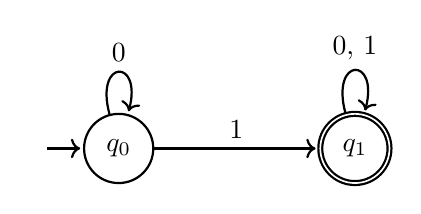
\begin{tikzpicture}[shorten >=1pt,node distance=3cm,on grid,auto, thick]
       \node[state,initial,initial text=] (q0) {$q_0$};
       \node[state,accepting] (q1) [right=of q0] {$q_1$};

       \path[->] 
       (q0) edge [loop above] node {0} (q0)
            edge node {1} (q1)
       (q1) edge [loop above] node {0, 1} (q1);
    \end{tikzpicture}
    \caption{DFA Mengandung Minimal Satu "1"}
\end{figure}

\textbf{Simulasi Input $w = 0011$ (Diterima)}[cite: 2]:
\begin{itemize}
    \item $\delta(q_0, 0) = q_0$ (Loop pencarian, belum menemukan 1)[cite: 2].
    \item $\delta(q_0, 0) = q_0$ (Loop pencarian)[cite: 2].
    \item $\delta(q_0, 1) = q_1$ (Berpindah, "1" ditemukan)[cite: 2].
    \item $\delta(q_1, 1) = q_1$ (Loop stabilitas, tetap di accept state)[cite: 2].
    \item Karena berakhir di $q_1 \in F$, maka string \textbf{Diterima}[cite: 2].
\end{itemize}

\subsection{Contoh 2: DFA String Dimulai dengan "0"}
Misalkan $L(M) = \{ 0, 00, 01, 000, 010, \dots \}$[cite: 3].
Ini berarti huruf pertama \textit{wajib} 0. Jika huruf pertamanya 1, maka otomatis gagal selamanya.

\begin{figure}[h]
    \centering
    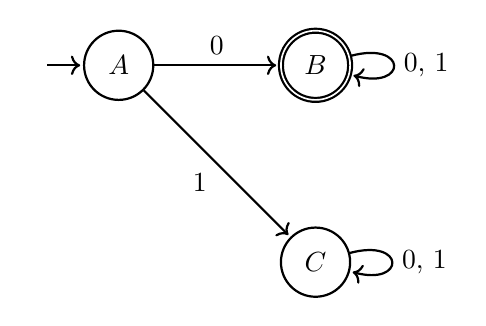
\begin{tikzpicture}[shorten >=1pt,node distance=2.5cm,on grid,auto, thick]
       \node[state,initial,initial text=] (A) {$A$};
       \node[state,accepting] (B) [right=of A] {$B$};
       \node[state] (C) [below=of B] {$C$};

       \path[->] 
       (A) edge node {0} (B)
           edge node [swap] {1} (C)
       (B) edge [loop right] node {0, 1} (B)
       (C) edge [loop right] node {0, 1} (C);
    \end{tikzpicture}
    \caption{DFA Dimulai dengan 0. State C bertindak sebagai Dead State.}
\end{figure}

\textbf{Simulasi Input $w = 101$ (Ditolak)}[cite: 3]:
\begin{itemize}
    \item $\delta(A, 1) = C$ (Huruf pertama salah, masuk ke Dead State)[cite: 3].
    \item $\delta(C, 0) = C$ (Terjebak di Dead State)[cite: 3].
    \item $\delta(C, 1) = C$ (Terjebak di Dead State)[cite: 3].
    \item Karena berakhir di $C \notin F$, maka string \textbf{Ditolak}[cite: 3].
\end{itemize}

\subsection{Contoh 3: DFA Panjang String Persis 2}
Misalkan $L(M) = \{00, 01, 10, 11\}$, dengan alfabet $\Sigma = \{0, 1\}$[cite: 3].

\begin{figure}[h]
    \centering
    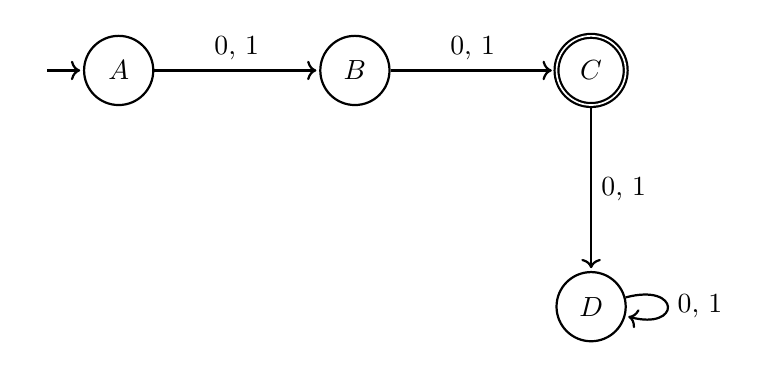
\begin{tikzpicture}[shorten >=1pt,node distance=3cm,on grid,auto, thick]
       \node[state,initial,initial text=] (A) {$A$};
       \node[state] (B) [right=of A] {$B$};
       \node[state,accepting] (C) [right=of B] {$C$};
       \node[state] (D) [below=of C] {$D$};

       \path[->] 
       (A) edge node {0, 1} (B)
       (B) edge node {0, 1} (C)
       (C) edge node {0, 1} (D)
       (D) edge [loop right] node {0, 1} (D);
    \end{tikzpicture}
    \caption{DFA Panjang Tepat 2. State D bertindak sebagai Dead State.}
\end{figure}

Pada kasus ini, langkah komputasinya sangat linier. Mesin hanya menerima string jika setelah membaca tepat dua karakter, mesin berhenti[cite: 3]. Jika ada karakter ketiga yang dibaca, mesin akan langsung pindah ke state D (\textit{Dead State}) dan menolak string tersebut selamanya[cite: 3].

\subsection{Contoh 4: Evaluasi Pola String yang Rumit}
Kita uji DFA dengan fungsi perluasan $\delta^*(q_0, w)$ menggunakan definisi pada tabel transisi Contoh 3 sebelumnya (dengan state $q_0, q_1, q_2$)[cite: 3].
Alfabet $\Sigma=\{a,b\}$, $F=\{q_0, q_1\}$.

\begin{figure}[h]
    \centering
    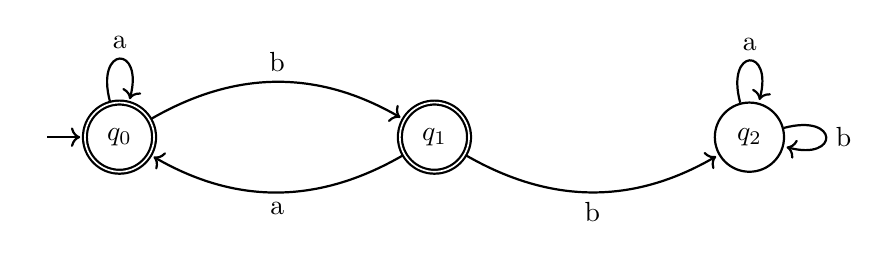
\begin{tikzpicture}[shorten >=1pt,node distance=4cm,on grid,auto, thick]
       \node[state,initial,initial text=,accepting] (q0) {$q_0$};
       \node[state,accepting] (q1) [right=of q0] {$q_1$};
       \node[state] (q2) [right=of q1] {$q_2$};

       \path[->] 
       (q0) edge [loop above] node {a} (q0)
            edge [bend left] node {b} (q1)
       (q1) edge [bend left] node {a} (q0)
            edge [bend right] node [swap] {b} (q2)
       (q2) edge [loop above] node {a} (q2)
            edge [loop right] node {b} (q2);
    \end{tikzpicture}
    \caption{DFA Pola Bahasa. State $q_2$ adalah Dead State.}
\end{figure}

\textbf{Tracing Input $w = abababaa$}[cite: 3]:
Langkah-langkah evaluasinya diselesaikan dari kiri ke kanan dengan menurunkan fungsi transisi yang diperluas:
\begin{enumerate}
    \item $\delta^*(q_0, abababaa) \Rightarrow \delta(q_0, a)$ menghasilkan $q_0$, sisa string: $bababaa$[cite: 3].
    \item $\Rightarrow \delta^*(q_0, bababaa) \Rightarrow \delta(q_0, b)$ menghasilkan $q_1$, sisa string: $ababaa$[cite: 3].
    \item $\Rightarrow \delta^*(q_1, ababaa) \Rightarrow \delta(q_1, a)$ menghasilkan $q_0$, sisa string: $babaa$[cite: 3].
    \item $\Rightarrow \delta^*(q_0, babaa) \Rightarrow \delta(q_0, b)$ menghasilkan $q_1$, sisa string: $abaa$[cite: 3].
    \item $\Rightarrow \delta^*(q_1, abaa) \Rightarrow \delta(q_1, a)$ menghasilkan $q_0$, sisa string: $baa$[cite: 3].
    \item $\Rightarrow \delta^*(q_0, baa) \Rightarrow \delta(q_0, b)$ menghasilkan $q_1$, sisa string: $aa$[cite: 3].
    \item $\Rightarrow \delta^*(q_1, aa) \Rightarrow \delta(q_1, a)$ menghasilkan $q_0$, sisa string: $a$[cite: 3].
    \item $\Rightarrow \delta^*(q_0, a) \Rightarrow \delta(q_0, a)$ menghasilkan $q_0$ (String habis)[cite: 3].
\end{enumerate}
Karena \textit{tracing} berakhir tepat pada state $q_0$ dan $q_0 \in F$ (State AKHIR), maka kalimat $abababaa$ dinyatakan \textbf{Diterima}[cite: 3].
Dapat disimpulkan bahwa bahasa $L(M)$ ini menerima string seperti $abababaa$, $aaabab$, $aabababa$, selama tidak menjumpai kombinasi substring "bb" yang memicu perpindahan ke dead state $q_2$[cite: 3].

\end{document}